
\documentclass[legalpaper, 12pt, addpoints, answers]{exam}
\usepackage[margin=1in]{geometry}
\usepackage[utf8]{inputenc}
\usepackage{graphics}
\usepackage{color}
\usepackage{amssymb}
\usepackage[spanish]{babel}
\usepackage{amsmath}
\usepackage{enumitem}
\usepackage{xcolor}
\usepackage{cancel}
\usepackage{ragged2e}
\usepackage{graphicx}
\usepackage{multicol}
\usepackage{color}
\usepackage{tikz}

%\CorrectChoiceEmphasis{\itseries\color{red}}

 
\everymath={\displaystyle}
\renewcommand*{\choicelabel}{(\thechoice)}
\renewcommand*{\choicelabel}{ 
  \ifnum\value{choice}>1
    \makebox[4em][r]{(\thechoice)}
  \else
    (\thechoice)
  \fi
}

\setlength{\multicolsep}{0.6em}
\begin{document}

%\begin{figure}[t]
%\includegraphics[width=1\textwidth,height=1.2\textheight,keepaspectratio]{header-cufm.png}
%\end{figure}

\begin{center}
Fall 2018 \\
\textbf{Midterm Exam} \\
Language Acquisition \\
LNG 230/SPV 221
\end{center}
\extraheadheight{-0.5in}


\runningheadrule \extraheadheight{0.1in}

\vspace{0.15in}
\runningheadrule \extraheadheight{0.14in}

\lhead{\ifcontinuation{Pregunta \ContinuedQuestion\ continua\ldots}{}}
\runningheader{Language Acquisition }{Midterm}{Fall 2018}
\runningfooter{Lehman College}
              {\thepage\ of \numpages}
              {LNG 230/SPV 221}
\vspace{0.15in}

\nopointsinmargin
\setlength\linefillthickness{0.1pt}
\setlength\answerlinelength{0.1in}
\vspace{0.25in}
\parbox{6in}

\parbox{6in}{\textsc{{}}
\vspace{0.15in}

\parbox{5in}{
{\textsc{\textbf{Part I.} Multiple Choices}}}}

\vspace{0.15in}
\hrule 
\vspace{0.15in}
\begin{questions}


\setlength{\multicolsep}{0.5em}
    \question Writers can use language to create a fictional world about future. This reflects which feature of language:
    
        \begin{choices} 
            \choice  Semanticity
            \choice  Arbitariness
            \choice  Productivity
            \choice  Displacement
        \end{choices}
        \vspace{0.15in}

\question In a language acquisition experiment, the children were asked to match the picture to the sentences they just heard. What method is used?

    \begin{choices}
            \choice Truth Value Judgment
            \choice Picture Matching
            \choice Act-Out Task
            \choice Naturalist experiment
    \end{choices}
    \vspace{0.15in}

    \question What is ERP?
    
    \begin{choices}
            \choice Event-related Possibilities
            \choice Event-regulated Potentials
            \choice Event-related Potentials
            \choice Event-regulated Possibilities 
    \end{choices}
    \vspace{0.15in}

     \question Calculate MLU of utterances below:\\
     \textit{
     206	*CHI:	stop .\\
     207	*CHI:	Mommy (.) I going get me some water .\\
     208	*CHI:	I wonder if [?] cookies could stop it .\\ 
     209	*CHI:	could stop it .\\
     210	*CHI:	cookies .\\}
     
        \begin{oneparchoices}
            \choice \(3.67\)
            \choice \(4.4\)
            \choice \(4\)
            \choice \(3.33\)
        \end{oneparchoices}
\vspace{0.15in}
    
\question Which theory does not explain how children identify meaning sounds in speech?

        \begin{choices}
            \choice Attuenment Theory
            \choice Transitional Probability
            \choice Motor Theory
            \choice Universal Theory
        \end{choices}
        \vspace{0.15in}

        \question If a child thought the word "atomic" is actually two words "a tomic", which cue did the child use to segment \textit{atomic}
        
   \begin{choices}
            \choice Phonotactic regularities
            \choice Prosodic Cues
            \choice Allophones
            \choice Refernce cues
\end{choices}
        \vspace{0.15in}

        \question What is a marked sound in English?
        
   \begin{oneparchoices}
            \choice /a/
            \choice /b/
            \choice /th/
            \choice /v/
   \end{oneparchoices}
        
        \vspace{0.15in}

        \question Which two sounds are allophones?

\setlength{\multicolsep}{0.5em}
        \begin{choices}
            \choice 't' in  Water and Table
            \choice 'a' in apple and amazing
            \choice 'th' in that and Thai
            \choice 'i' in big and ship
        \end{choices}
        \vspace{0.15in}
        
\setlength{\multicolsep}{0.5em}
         \question What is the physical structure that enables human to make sounds?
         
    \begin{choices}
            \choice larynx
            \choice tongue
            \choice vocal tract
            \choice mouth
   \end{choices}
        \vspace{0.15in}

            \question When a child wants to say "puddle", he/she says "puggle". However when he/she tries to say "puzzle", he/she says "puddle". Which theory can not explain this?
        \begin{choices}
            \choice Articulatory constraints
            \choice Universal Constraints
            \choice Mispronounciation due to misperception
            \choice Template Theory
        \end{choices}
         \vspace{0.15in}    
        \question In the gavagai scenario, which can be the meaning of gavagai?
        
 \begin{choices}
            \choice rabbit
            \choice hunt
            \choice pay attention
            \choice all above
\end{choices}
        \vspace{0.15in}
         
            \question The child can recognize chihuahua as a dog but refuses to call Snoopy a dog. Which might be the reason?
        \begin{choices}
            \choice The child doesn't like Snoopy.
            \choice Snoopy looks different from a chihuahua.
            \choice The child failed to extend the concept 'dog' to nonanimate cartoon image
            \choice Snoopy is not a real dog
        \end{choices}
        \vspace{0.15in}

\question In an ERP study, the child reads sentences on the screen. Which ERP component should we expect when the child reads an ungrammatical sentence?

    \begin{oneparchoices}
         \choice N600
         \choice N400
         \choice P600
         \choice P400
    \end{oneparchoices}
\vspace{0.2in}

\question When a child reads Garfield comic book, he/she knows that Garfield and cat all refer to the protagonist of the comic book. This would be a counter-example of which theory:

%%%%%% ---Comment out to add a header image ----
%\begin{figure}[h]
%\begin{center}
%\includegraphics[width=0.5\textwidth,height=1\textheight,keepaspectratio]{prisma.png}
%\end{center}
%\end{figure}

        \begin{choices}
            \choice Whole Item Assumption
            \choice mutual exclusivity assumption
            \choice The taxonomic assumption
            \choice The shape bias:
        \end{choices}
  \vspace{0.15in}

 \question English children usually acquire /a/ sound earlier than /th/ sound, which could be an explanation for this?
 
        \begin{choices}
            \choice /a/ is an unmarked sound, /th/ is a marked sound. Children acquire unmarked sounds faster than marked ones.
            \choice /a/ is a marked sound, /th/ is an unmarked sound. Children acquire marked sounds faster than unmarked ones.
            \choice /a/ is a vowel and /th/ is a consonant. Children acquire vowels faster than consonant.
            \choice /a/ appears in 'mama', which is the first word the children produce. 
        \end{choices}
\vspace{0.15in}

 \question In order to collect data, the researcher decides to go to a family and record all the interaction and conversation, what type of data is collected and which method is this? 
 
        \begin{choices}
            \choice production, experiment
            \choice comprehension, naturalistic
            \choice production, naturalist
            \choice comprehension, experiment
        \end{choices}
\vspace{0.15in}

\question Calculate MLU of children's utterances below:\\
91  *CHI:	you play another game with me .\\
92	*CHI:	what you making .\\
93	*MOT:	I'm writing .\\
94	*CHI:	why you writing ?\\
95	*MOT:	I always write when I come (.) don't I ?\\
96	*CHI:	yep .\\
97	*CHI:	down here .\\
98	*MOT:	is that right ?\\
99	*CHI:	yeah .\\


        \begin{oneparchoices}
        \choice 1.8
        \choice 3
        \choice 2.67
        \choice 3.33
        \end{oneparchoices}
\vspace{0.10in}

\question What are the circles and lines in the picture?

\begin{choices}
      \choice fixation, saccade
      \choice gaze, saccade
      \choice fixation, rapid eye movement
      \choice gaze, rapid eye movement
\end{choices}
   \begin{figure}[h]
        \centering
        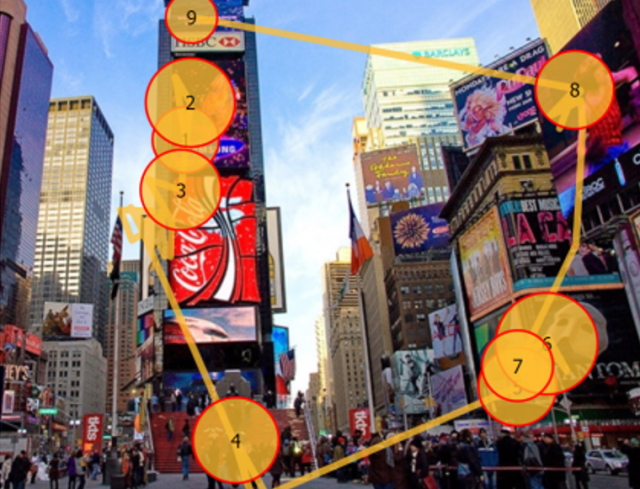
\includegraphics[height = 6cm, width = 8cm]{Fixation-sequences.png}
    \end{figure}
    
\vspace{0.10in}

\question Which of the following is not one morpheme in counting MLU?

\begin{oneparchoices}
    \choice gonna
    \choice whom
    \choice went
    \choice John's
\end{oneparchoices}
\vspace{0.10in}
\question Which is a more likely age for children to say their first words?

\begin{oneparchoices}
      \choice 15 months
      \choice 25 months
      \choice 35 months
      \choice 5 months
\end{oneparchoices}
\vspace{0.10in}
\question Why speech segmentation is a difficult task for infants?

\begin{choices}
      \choice Adults talk too fast.
      \choice Infants don't know how to spell words
      \choice There is no reliable acoustic gap to signal words.
      \choice The sentences are too long for infants to segment.
\end{choices}
\question We have a limit set of alphabet but we can make infinite sentences out of it. This reflects which feature of language?

\begin{choices}
      \choice Semanticity
      \choice Arbitariness
      \choice Productivity
      \choice Displacement
\end{choices} 
\question Syntactic Priming is a type of...

\begin{choices}
      \choice Naturalisitic study 
      \choice Truth Value Judgment
      \choice Production experiment
      \choice Word Acquisition study
\end{choices} 

\question This is a picture of which study?
    \begin{figure}[h]
        \centering
          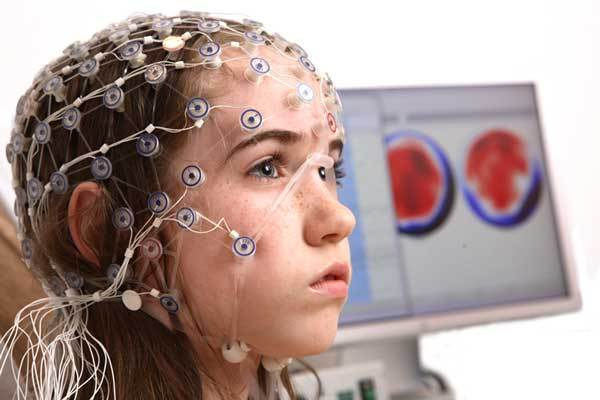
\includegraphics[height = 6cm, width = 8cm]{global-adult-eeg-cap-market-1.jpg}
        \end{figure}

\begin{choices}
      \choice eye-tracking
      \choice naturalistic study
      \choice ERP
      \choice brain wave study
\end{choices} 

\question Which statement is correct about speech recognition

\begin{choices}
      \choice Infants learn the phonemes in their native language first and they are not sensitive to the phonemes there are not in their native language
      \choice Infants can not differentiate speech sound and noise
      \choice Father's voice and mother's voice are the same to infants
      \choice Speech Pattern Recognition starts prenatal
\end{choices} 


\pagebreak
\parbox{5in}{
{\textsc{\textbf{Part II.} Short Essay Questions}}}

\vspace{0.10in}




\question What are the features of Infants Vocalization? 





\question Explain what is reference problem and extension problem in word acquisition.



\question What cues do children use to segment speech? Give an example of each cue.

\vspace{0.15in}

\parbox{5in}{
{\textsc{\textbf{Part II.} Long Essay Questions}}}

\vspace{0.10in}

Choose one to answer

\question 2 y/o Adam is playing with his mother. Mother showed Adam a teddy bear and said "teddy bear". Adam learned the word "teddy bear". However, when Adam saw a brown poodle dog, he pointed at the poodle dog and said "teddy bear". Use this example to explain at least three the concepts listed below. 
\\
\textbf{Concepts:} joint attention; communicative intent; associative learning; whole item assumption; shape bias; reference; extension


\question Sarah is 2 y/o. She makes many errors in her utterances. She would say "raser" instead of "eraser", "tato" instead of "potato". Also, she would call "pizza" as "pita", "Lisa" as "Lita". Please provide at least three explanations for Sarah's errors.

\end{questions}
\end{document}
  